\chapter{Experimental evaluation} \label{sec:experimentsoutside}
The simulations conducted in the previous chapter form the basis for real world measurements and experimental evaluation of the MP-SRP-PHAT algorithm, and to test its performance and robustness in various conditions. In order to test the algorithm under ideal, controlled conditions, anechoic measurements were conducted. After that a series of outdoor sources and environments were tested. This chapter contains the results of the experiments. 

\section{Microphone array and acquisition system}
The equipment used for the experiments are listed below.
\begin{table}[!ht]
    \centering
	\begin{tabular}{ll} \toprule
	{Item \#}	&	{Description}\\
	    \bottomrule 
	        &   \textbf{{General}}                                       \\
	    1   &   4 B\&K  Type 4935 microphones                            \\
	    2   &   1 B\&K Module Type 3050-A-060 interface module           \\
	    3   &   Prototype tetrahedral microphone stand                   \\
		4   &   PC with MATLAB, Python and B\&K Pulse software           \\
		5   &   Relevant cables and wires                                \\
		\bottomrule 
            &  \textbf{{Anechoic measurements}}                           \\
		6	&   1 B\&K OmniPower loudspeaker                              \\
		7   &   2 custom spherical speakers                               \\
		8   &   1 Pioneer A-656 amplifier                                 \\
		9   &   1 B\&K Type 2270 hand-held analyzer                       \\
		\bottomrule 
		    &   \textbf{{Outdoor measurements}}                           \\
		10  &   1 B\&K Module Type 2831 battery module                    \\
		11  &   4 B\&K microphone ellipsoidal windscreens                  \\
		\bottomrule 
	\end{tabular}
\end{table}
A prototype microphone array structure was used to record sound sources, on which 4 B\&K Type 4935 microphones could be placed in a tetrahedral configuration (Fig. \ref{fig:arraymic1}). The 4 microphones were mounted on the array vertically (pointing upwards). The microphones could be placed between 10cm-1m to each other in discrete steps. The middle vertical rod of the structure was placed on a tripod. The height of the array could be adjusted by moving the middle rod up-down, and also by adjusting the tripod height. During the measurements, the array was kept horizontally, such that three of the microphones were on the same horizontal plane. For the outdoor measurements, the array was kept as high as possible, such that the base of the array was $\approx1.5m$ above the ground. B\&K Pulse software suite was used for recording. B\&K Module Type 3050-A-060 was used as the main interface sound card and microphones were plugged into it with BNC connectors. During outside measurements, foam microphone windscreens were mounted on the microphones and a B\&K battery module was used to power the soundcard. The recordings were converted to 16bit .wav files, recorded with a sampling rate of 131072Hz (the maximum sampling rate available on the system). Two different values of the tetrahedral array aperture were used, 1m and 39.5cm, resulting in two different sizes for the tetrahedral array, large and small.
\begin{figure}
    \centering
    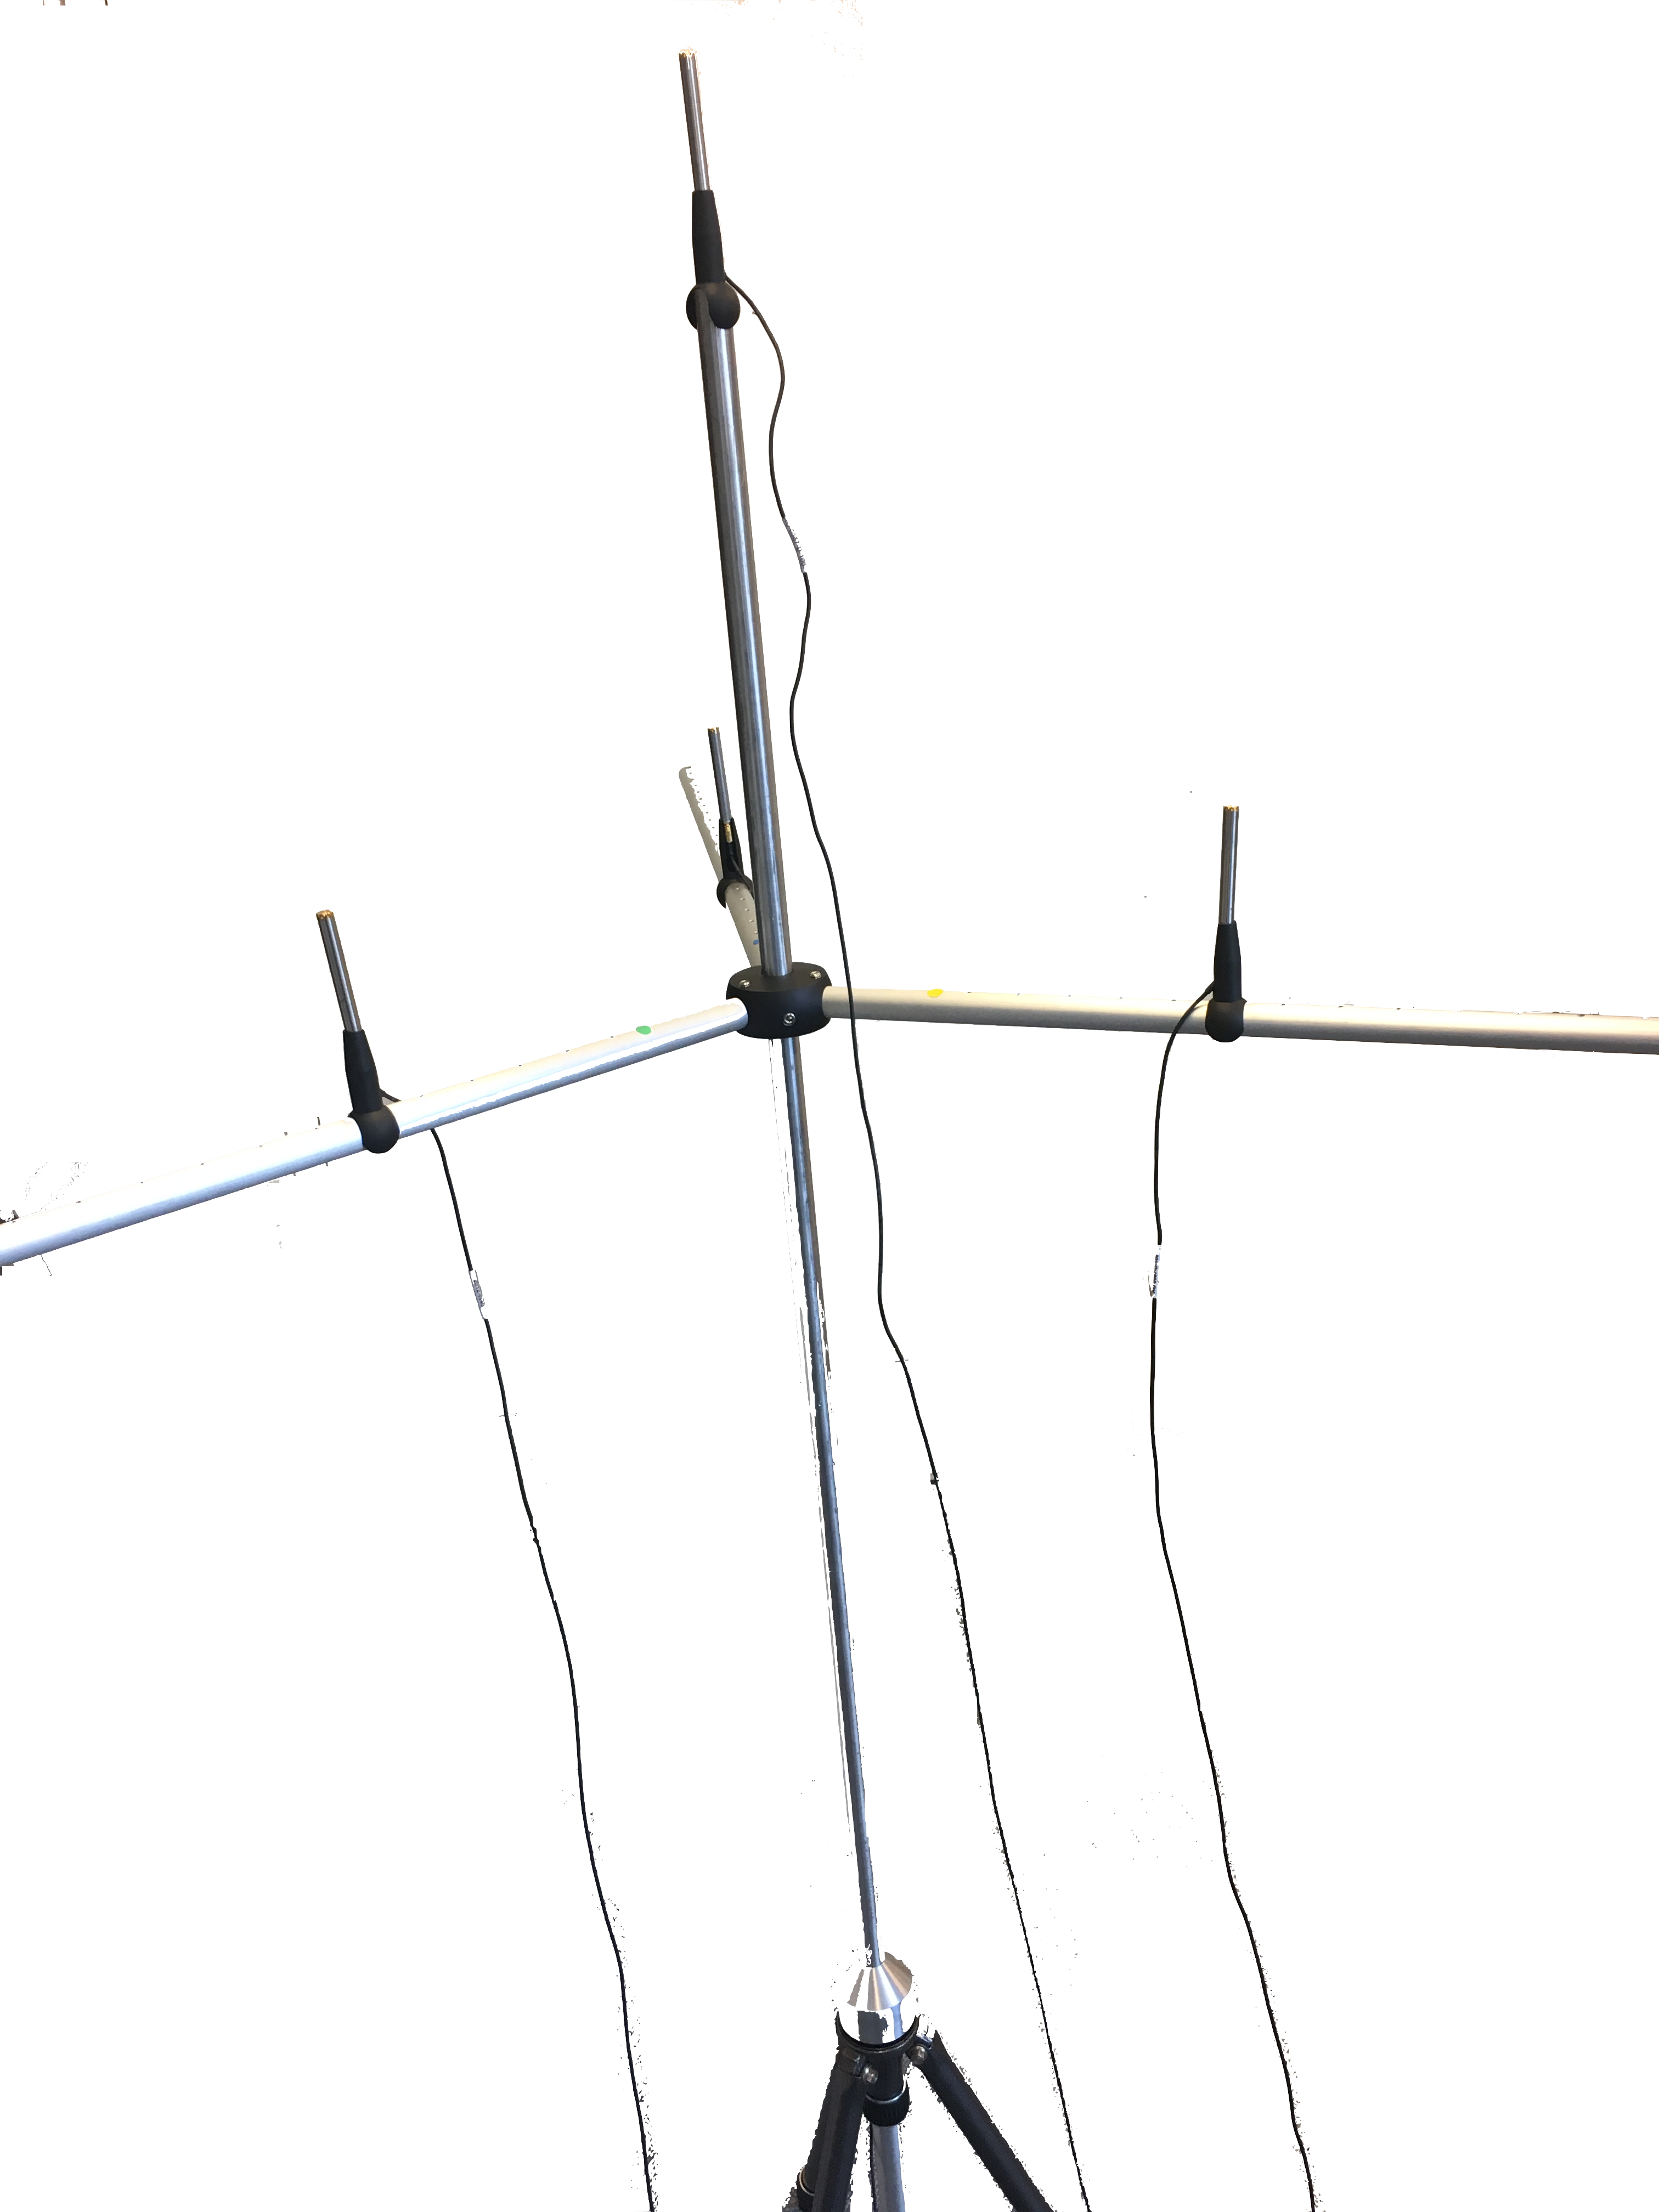
\includegraphics[width=0.4\textwidth]{Figures/Arraymicrophone.png}
    \caption{\label{fig:arraymic1}Prototype tetrahedral array used for measurements}
\end{figure}
\section{Anechoic Measurements}
The purpose of the anechoic measurements is to validate the MP-SRP-PHAT algorithm in a controlled environment. The criteria that are required to be validated are,
\begin{itemize}
    \item For a single source, the location is computed correctly.
    \item For multiple sources playing simultaneously, the locations are computed correctly.
    \item The relative levels of multiple sources are maintained.
    \item The actual levels of multiple sources are computed correctly.
\end{itemize}
\subsection{Experiment 1: Localizing a single sound source}
Pink noise from a single loudspeaker was recorded with the array\footnote{A recording of 300Hz sinusoidal wave was also performed to display the delays between the microphones (Appendix. \ref{add_Meas_1})}. The source was a B\&K Omnisource Type 4296 speaker with operating frequency of 100Hz-5kHz. Two separate measurements were done. For the first measurement, the loudspeaker was placed at (90$\degree$, 0$\degree$). For the second measurement, the loudspeaker position was kept the same and the microphone array was rotated $\approx$20$\degree$ around its axis in order to change the relative location (azimuth) of the speaker. The setup is described by Fig. \ref{fig:Anechoic1} where the source positions for the two measurements are shown. In order to approximate plane wave propagation, in the limited space of the anechoic chamber, the array was placed as far away from the source as possible and the array aperture was reduced to 0.395m. Temperature of the lab was 22 $\degree$C.
\begin{figure}[H]
    \centering
    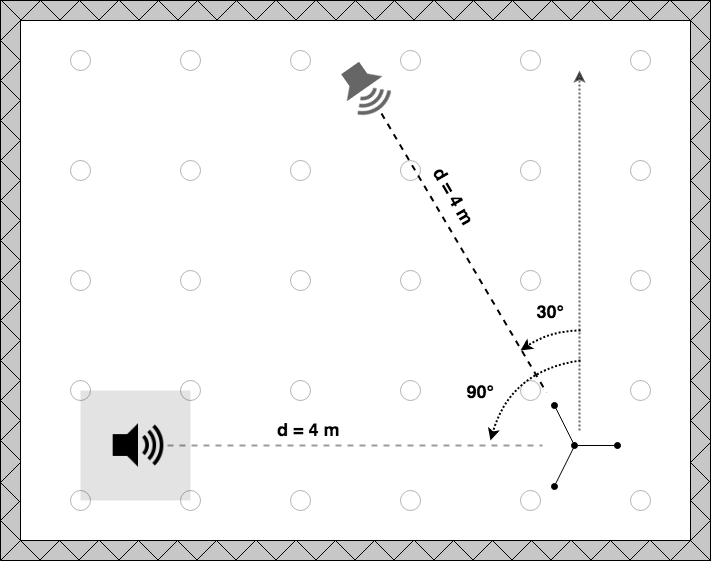
\includegraphics[width=0.6\textwidth]{Figures/Anechoicexp1.png}
    \caption{Sketch of the experiment.}
    \label{fig:Anechoic1}
\end{figure}
\subsubsection{Results}
The energy maps of the SRP-PHAT and minimum power SRP-PHAT algorithms are computed and displayed in Fig. \ref{fig:1srcAnechoic}. The source peak was localized at (89$\degree$, 0$\degree$) for both AM-SRP-PHAT and MP-SRP-PHAT. The error of 1$\degree$ in localization of the speaker is attributed to errors in placement. Fig. \ref{fig:1srcAnechoic} shows the results for source at (20 $\degree$, 0$\degree$). The source was localized to (23$\degree$, 0$\degree$) by both AM-SRP-PHAT and MP-SRP-PHAT. The azimuth error in localization of the speaker is attributed to errors in placement.
\begin{figure}[H]
    \centering
    \begin{subfigure}[b]{0.865\textwidth}
    \centering
    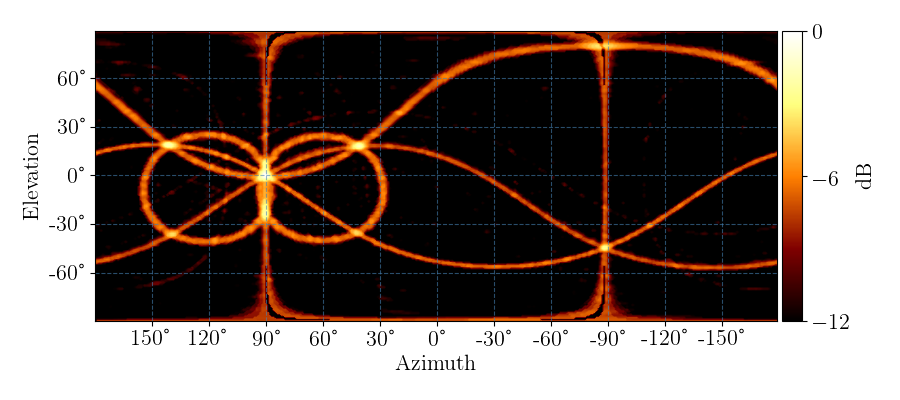
\includegraphics[width=0.865\textwidth]{Figures/Anechoic0Deg1SrcNorm.png}
\end{subfigure}
\vskip \baselineskip
\begin{subfigure}[b]{0.865\textwidth}
    \centering
    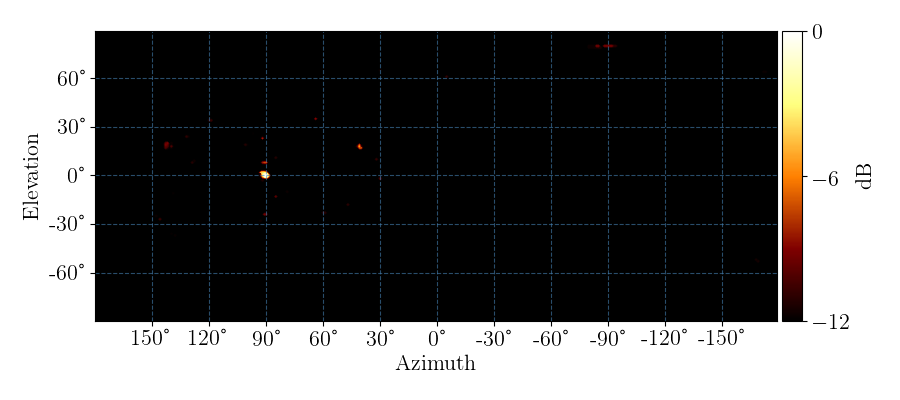
\includegraphics[width=0.865\textwidth]{Figures/Anechoic0Deg1SrcMinPow.png}
\end{subfigure}
\vskip \baselineskip
\begin{subfigure}[b]{0.865\textwidth}
    \centering
    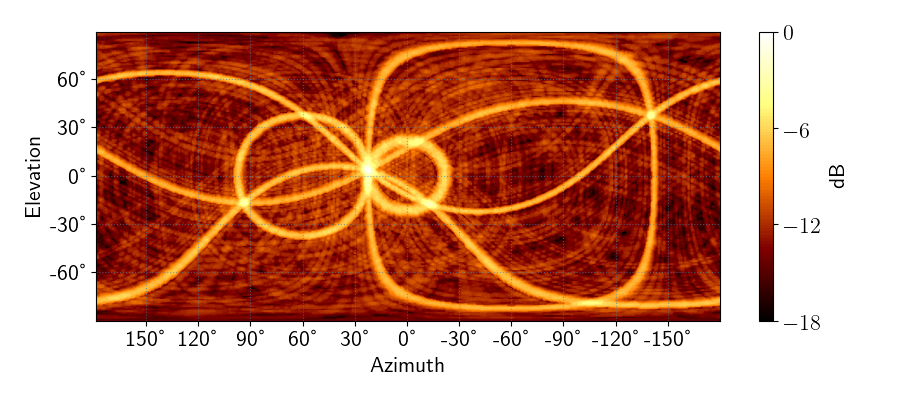
\includegraphics[width=0.865\textwidth]{Figures/Anechoic30Deg1SrcNorm.png}
\end{subfigure}
\vskip \baselineskip
\begin{subfigure}[b]{0.865\textwidth}
    \centering
    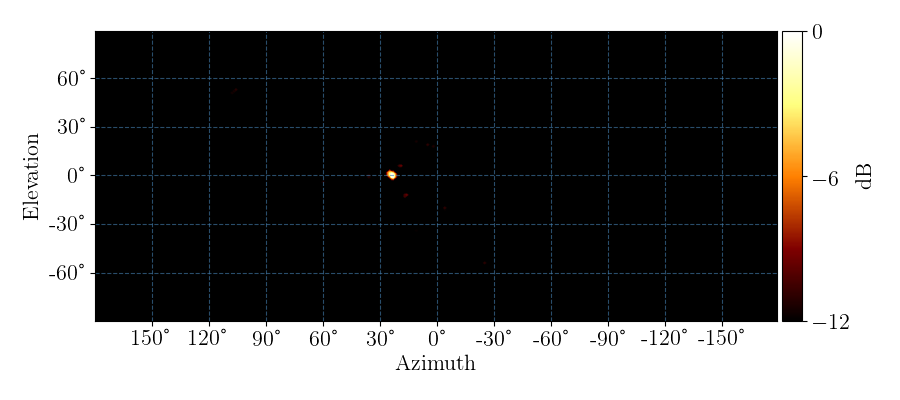
\includegraphics[width=0.865\textwidth]{Figures/Anechoic30Deg1SrcMinPow.png}
\end{subfigure}
\caption{Figures depict SRP-PHAT and minimum power SRP-PHAT localization for source around (90$\degree$,  0$\degree$) in an anechoic room (top 2), and for source at ($\approx$20$\degree$, 0$\degree$) in an anechoic room (bottom 2).}
\end{figure}
\subsection{Experiment 2: Localizing 2 sources and computing their levels}
 This experiment was run in the anechoic chamber to validate multiple source localization and retrieval of their relative sound level difference, as well as the absolute level of sources playing at the same time. Two custom spherical speakers were used to play the source signal and the aperture size of the array was set at 0.395m. One source was placed at (90$\degree$, 0$\degree$) and played pink noise at 46dB\footnote(The sound from each speaker was measured individually, using a level meter, at the array location.), the second source was placed at (130$\degree$, 0$\degree$) played uncorrelated pink noise at 52dB. The low frequencies (<200Hz) were filtered out in order to accommodate for the speakers used. Temperature of the room was recorded at 22$\degree$C.
\begin{figure}[H]
    \centering
    \includegraphics[width=0.8\textwidth]{Figures/AnechoicPic.jpg}
    \caption{Picture of the set up. The anechoic chamber was filled with misc. equipment, therefore the sources have been replaced by red dots for clarity. 90$\degree$ and 130$\degree$ azimuth are also drawn on top of the picture.}
    \label{fig:Anechoicpic1}
\end{figure}
\begin{figure}[H]
    \centering
    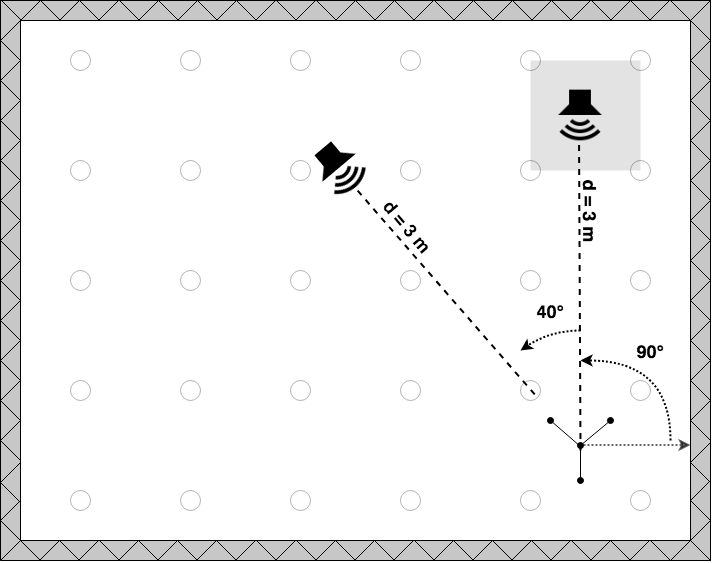
\includegraphics[width=0.6\textwidth]{Figures/Anechoicexp3.png}
    \caption{Sketch of the experiment}
    \label{fig:Anechoicexp3}
\end{figure}
\subsubsection{Results}
\begin{figure}[H]
    \centering
    \begin{subfigure}[b]{0.865\textwidth}
    \centering
    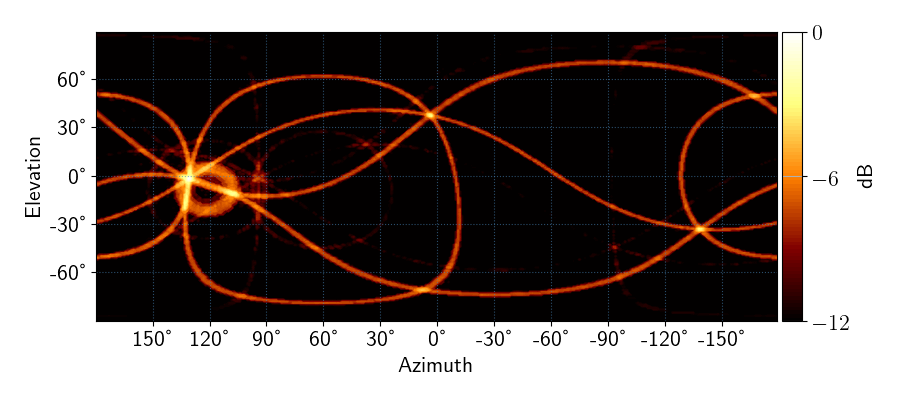
\includegraphics[width=0.865\textwidth]{Figures/Anechoic2SrcNorm.png}
\end{subfigure}
\vskip \baselineskip
\begin{subfigure}[b]{0.865\textwidth}
    \centering
    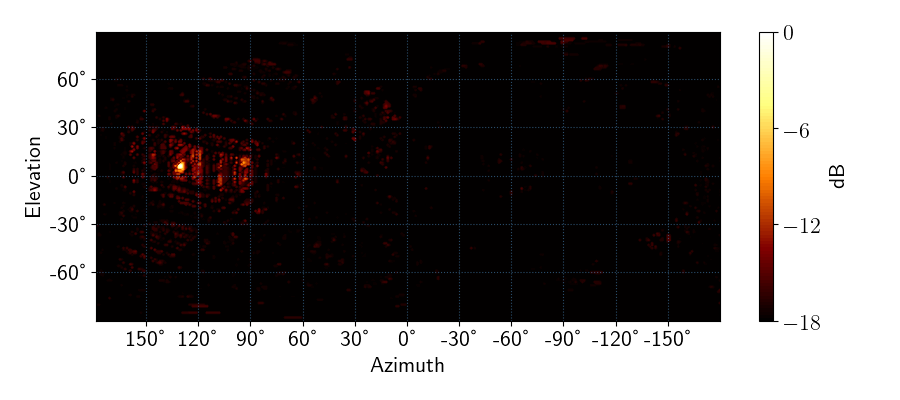
\includegraphics[width=0.865\textwidth]{Figures/Anechoic2SrcMinPow.png}
\end{subfigure}
\caption{Figure depicts SRP-PHAT (top) and minimum power SRP-PHAT (bottom) localization for 2 sources located at (90$\degree$, 0$\degree$) and (130$\degree$, 0$\degree$). The sources play uncorrelated pink noise at 52dB and 46dB respectively.}
\end{figure}
During the experiment, the anechoic chamber was not completely empty and some reflections can be observed at the 12dB dynamic range. Also, since the speakers were relatively close to the array, the cone approximation has larger errors. This can reduce the size of overlap of the multiple cones from the various microphones, or cause them to not overlap at all. This can be seen in the result for normal SRP-PHAT here, where the cones for the secondary cones barely overlap. Applying minimum power SRP-PHAT can then completely hide the secondary source. For this measurement however, the secondary source can be seen. The results from normal SRP-PHAT showed the secondary source level to be playing at -6.81dB relative to the main source. Understandably, due to the issues discussed here, the results for the MP-SRP-PHAT showed the secondary source level to be -8.18dB relative to the main source. Both AM-SRP-PHAT and MP-SRP-PHAT localized the peak of the main sound source at the same location (130$\degree$,-1$\degree$). The peak of the secondary source was localized at (95$\degree$,-2$\degree$) by  AM-SRP-PHAT and at (94$\degree$,-1$\degree$) by MP-SRP-PHAT. This minor difference can be attributed to the fact that the peak at (95$\degree$,-2$\degree$) was removed by the minimum power algorithm, due to no overlap at that location. The total power received at the array for the delay associated with the peak location was calculated according to Section \ref{srcLvlRetrieval}. It was computed to be 51.57dB. The results from here on will not be normalized to 0dB but shown as absolute source levels. 
\section{Outdoor measurements}
In order to test the algorithm in real conditions, several outdoor measurements in various conditions were conducted. Experiments were run in a construction field, in outdoor and indoor concerts, in traffic and in a chalk mining field. The recordings were done at the maximum sample rate available in the system, viz, 131072Hz. The microphone array aperture unless otherwise mentioned, was set at 1m, since the sources were always sufficiently far away for plane wave approximation to hold. Photos of the measured outdoor environment were taken using a camera having a known angle of view, such that the azimuth and elevation of the photos was known. Finally, the localization results were overlaid on the photos.
\subsection{Single static source on a construction field}
In this experiment, a single construction machine working in a fixed position was recorded by the microphone array. The source was more than 20 meters away. Fig. \ref{fig:Scenario1pic} describes the setup. The measurement system was set in the middle of a road, outside the construction field. There was a big office building with a smooth faćade behind the setup. Temperature was recorded at 23$\degree$C, speed of wind was 2m/s from (180$\degree$, 0$\degree$). Fig. \ref{Fig:OutdoorLast1Src} displays the full results.
\begin{figure}[H]
    \centering
    \hspace*{2.2cm}
    \begin{subfigure}[b]{0.85\textwidth}
    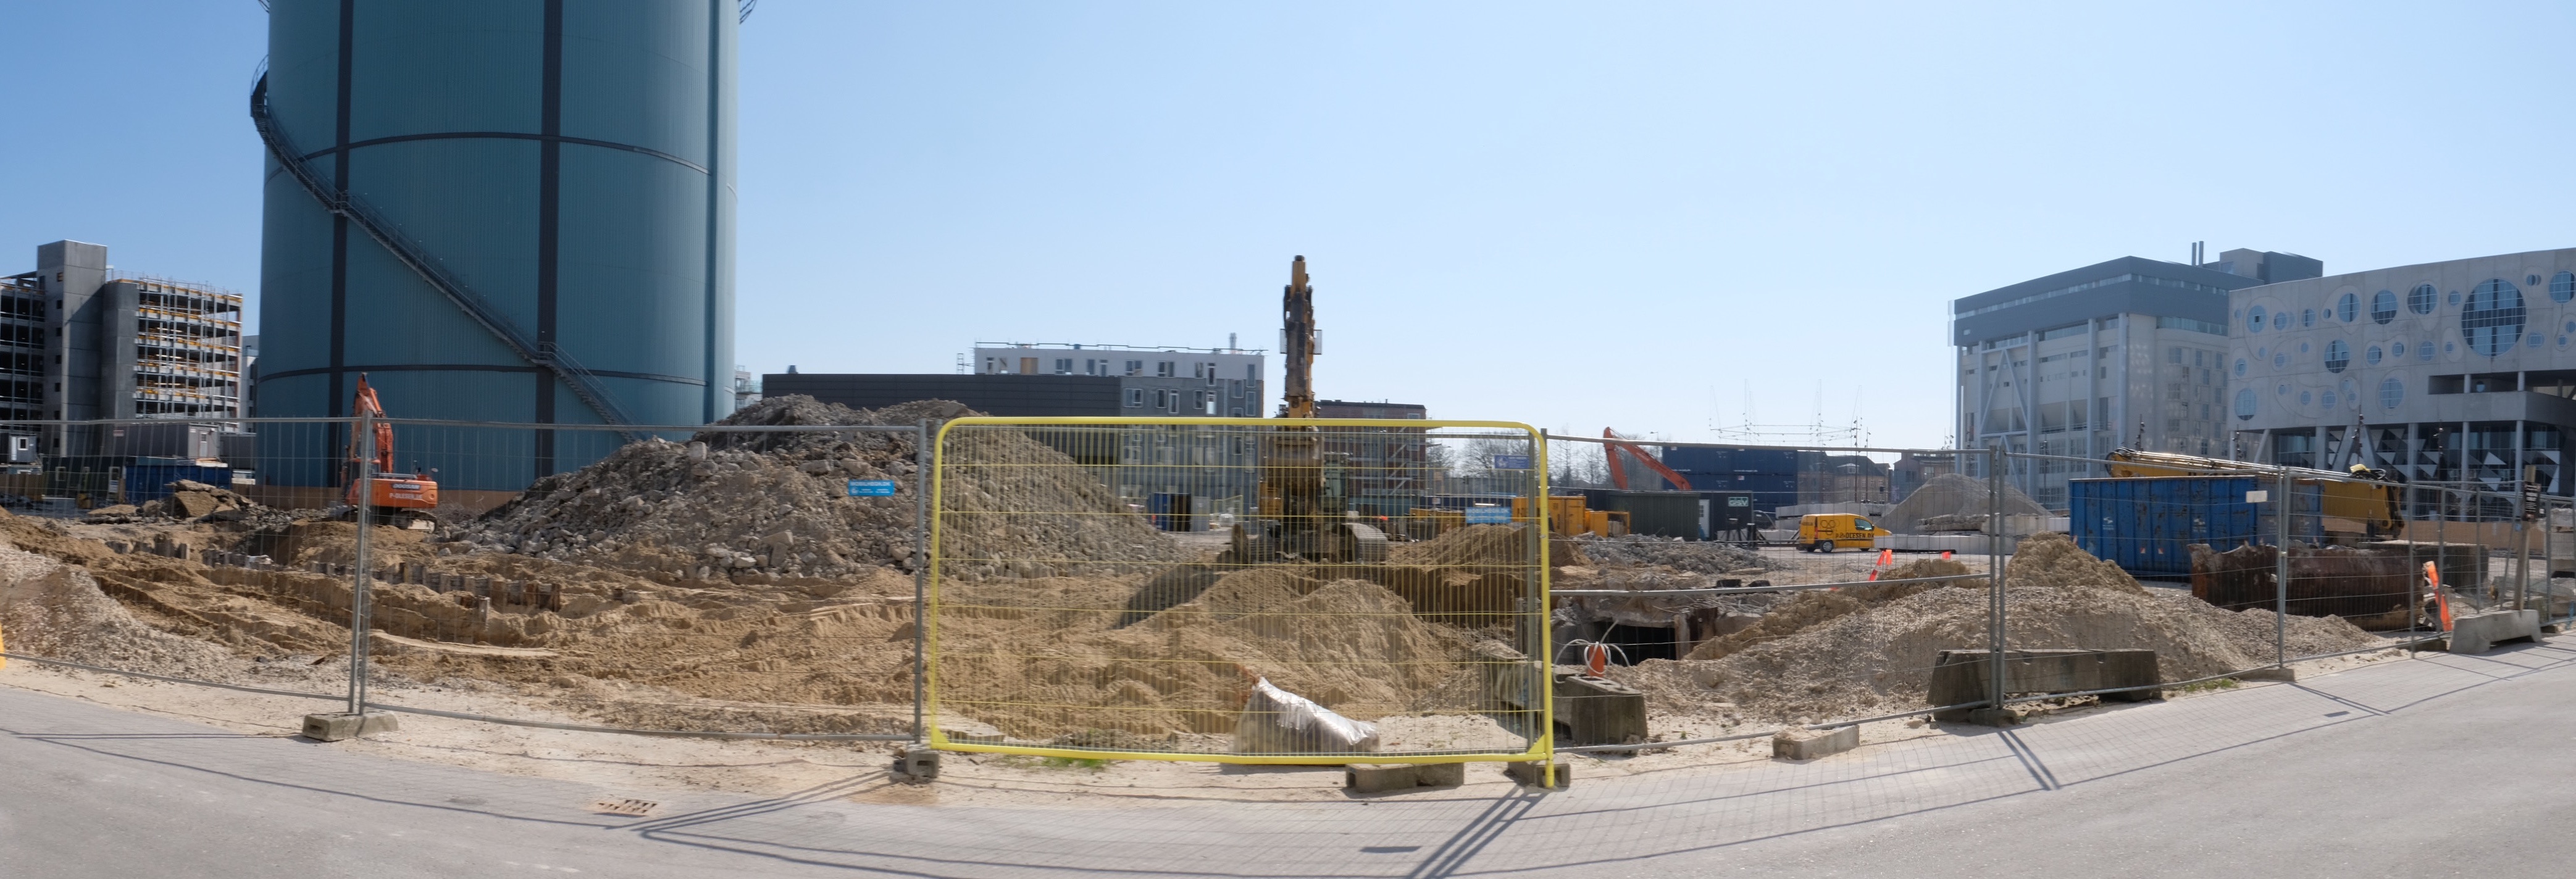
\includegraphics[width=0.85\textwidth]{Figures/Scenario1pic.jpg}
    \end{subfigure}
    \vskip \baselineskip
    \begin{subfigure}[b]{0.8\textwidth}
    \centering
    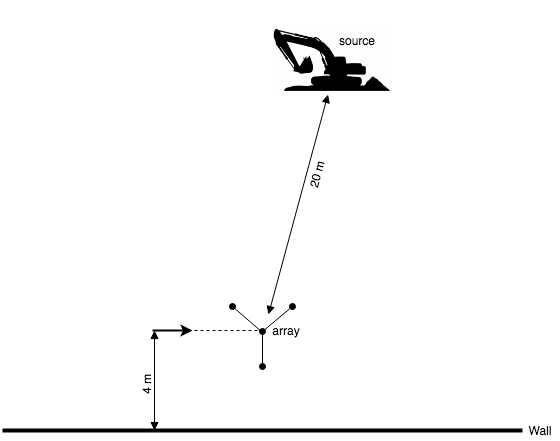
\includegraphics[width=0.8\textwidth]{Figures/scenario2diagram.png}
    \centering
    \end{subfigure}
    \caption{Figure shows the picture of the construction field (top) and the top view schematic of the construction field (bottom)}
    \label{fig:Scenario1pic}
\end{figure}
\subsubsection{Results}
\begin{figure}[H]
    \centering
    \begin{subfigure}[b]{0.865\textwidth}
    \centering
    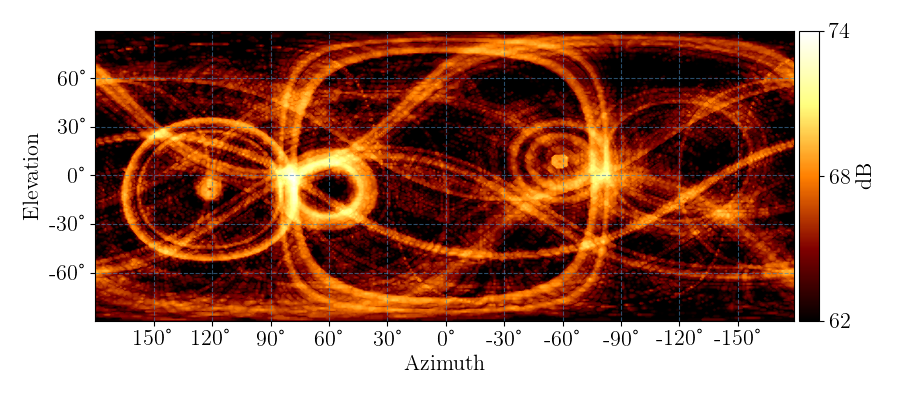
\includegraphics[width=0.865\textwidth]{Figures/construction2_normal.png}
\end{subfigure}
\vskip \baselineskip
\begin{subfigure}[b]{0.865\textwidth}
    \centering
    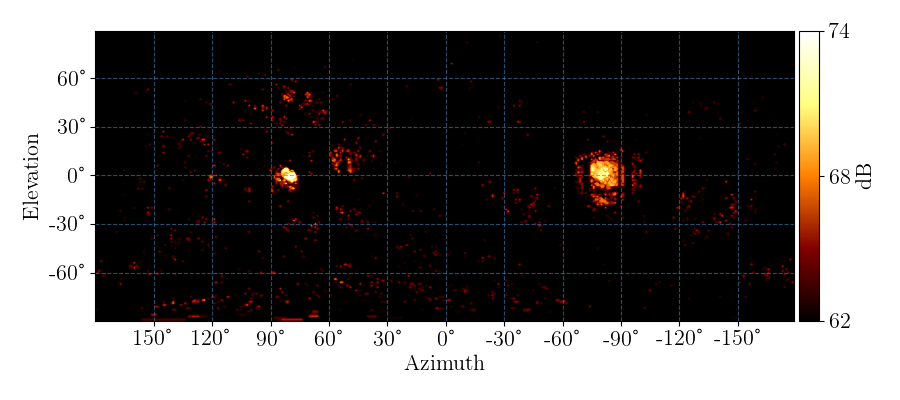
\includegraphics[width=0.865\textwidth]{Figures/construction2_minPow.png}
\end{subfigure}
\caption{Figures depict from top-to-bottom SRP-PHAT and minimum power SRP-PHAT localization for a single construction machine working in a construction field.}
\label{Fig:OutdoorLast1Src}
\end{figure}
As can be seen in the MP-SRP-PHAT result, 2 clear sources are visible at $\approx$($\pm$90$\degree$, 0$\degree$). The source at (90$\degree$, 0$\degree$) is the actual construction machine and the one at (-90$\degree$, 0$\degree$) can be attributed to its reflection from the office wall behind the array. The recordings were only 51sec long, the duration during which the machine was in the same location. The overlaid results are shown in Fig. \ref{Fig:overlayimageoutside2}. Even though the machine itself did not move, the excavator arm moved around the body of the machine emitting noise as it excavated. The sounds emitted at different positions around the motor due to the arm do not appear on the result. This is because the transient sounds averaged out over the duration of 51sec. 

However, as can be seen the result is fairly noisy. It is indeed difficult to get a clean map for a larger dynamic range in this reverberant field, as more and more reflections from the source become apparent. Other distant sources in the construction field and their own reflections also appear on the results. In addition, other noise sources such as the wind noise or other diffuse reflections might be appearing on the results, since some results can be seen with relatively high elevation, where no source was present. Taking longer recordings can help reduce these transient sounds from appearing on the results and improve achievable dynamic range.
\begin{figure}[!ht]
    \centering
    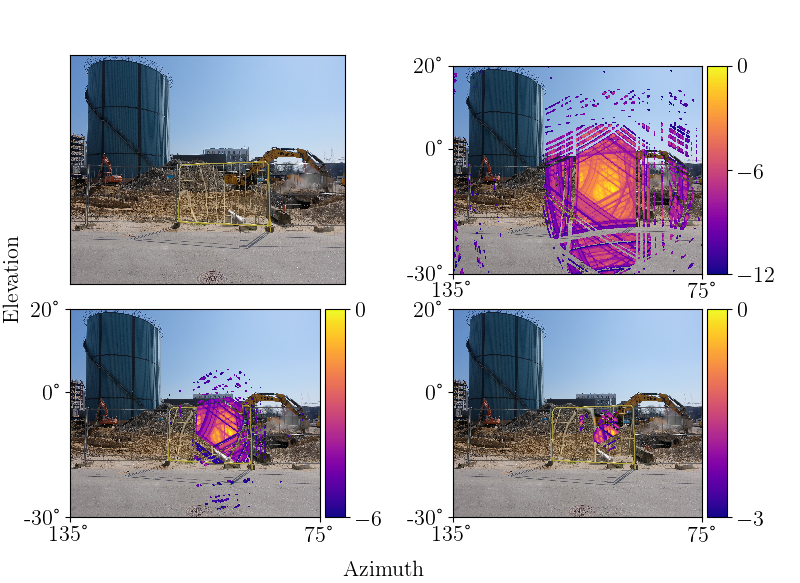
\includegraphics[width=0.96\textwidth]{Figures/const2image.png}
\caption{Figures depict localization results overlaid on the photo of the measured source with dynamic range of 12dB (top) and 6dB (bottom)}
\label{Fig:overlayimageoutside2}
\end{figure}
\subsection{3 static sources on a construction field}
In this experiment, 3 distinct noise sources were measured: a tapping machine in a hole in the ground located at (180$\degree$,<0$\degree$) and two excavators located between (120$\degree$,0$\degree$) and (150$\degree$,0$\degree$). Fig. \ref{fig:Scenario2} describes the setup. Fig. \ref{Fig:Outdoorpicfull} displays the results.
\begin{figure}[H]
    \centering
    \begin{subfigure}[b]{0.85\textwidth}
    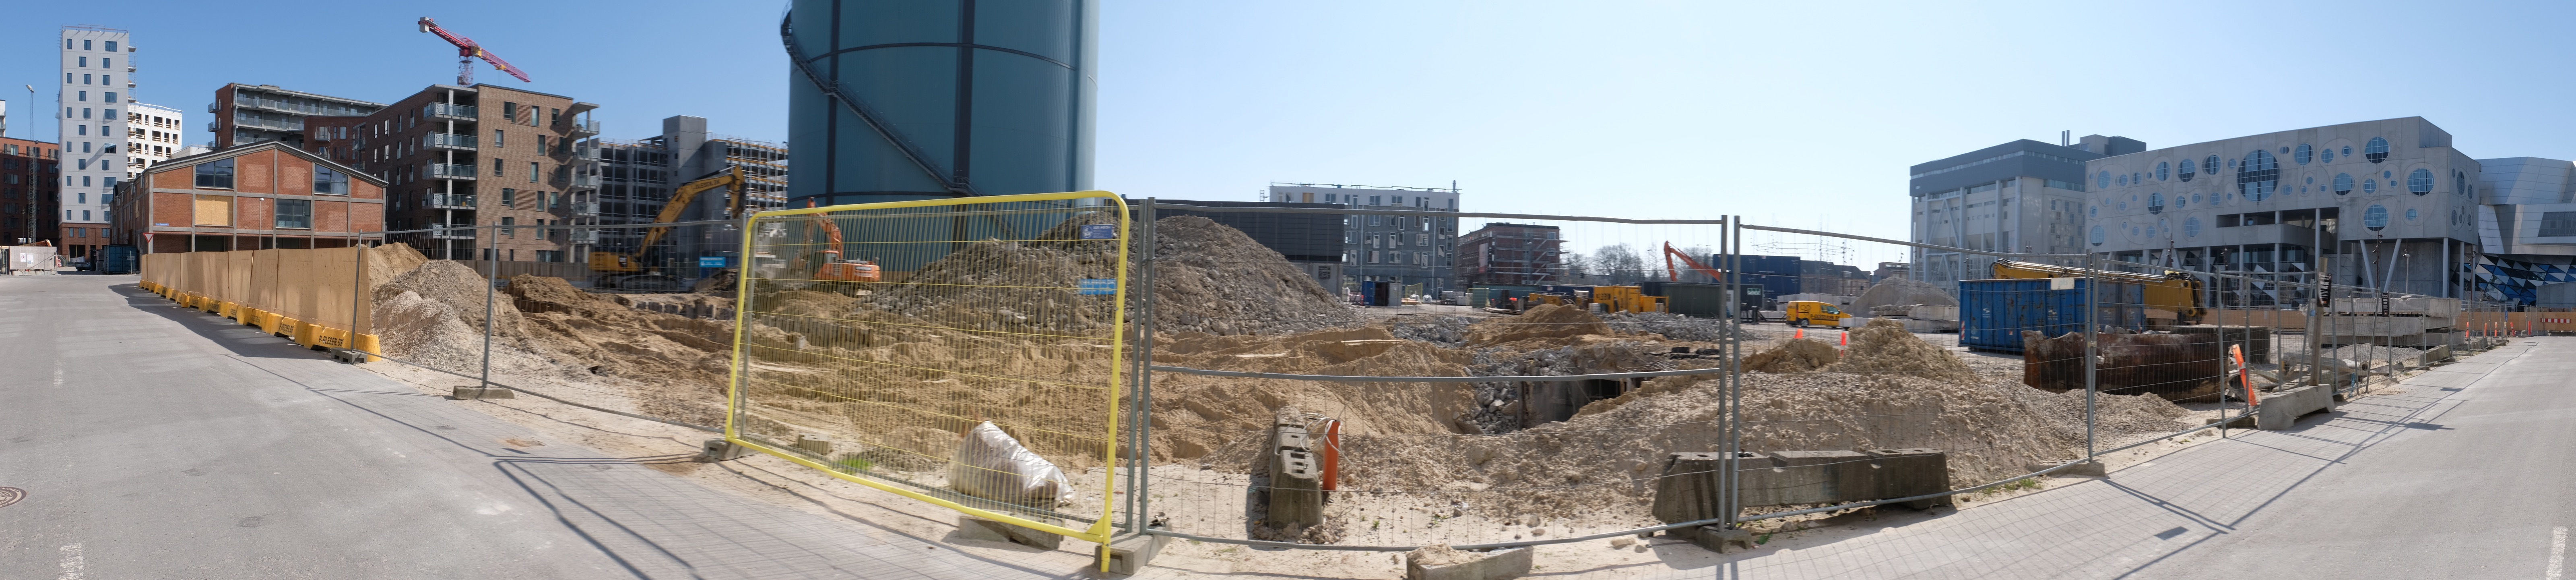
\includegraphics[width=0.85\textwidth]{Figures/scenario3pic.jpg}
    \end{subfigure}
    \vskip \baselineskip
    \begin{subfigure}[b]{0.8\textwidth}
    \centering
    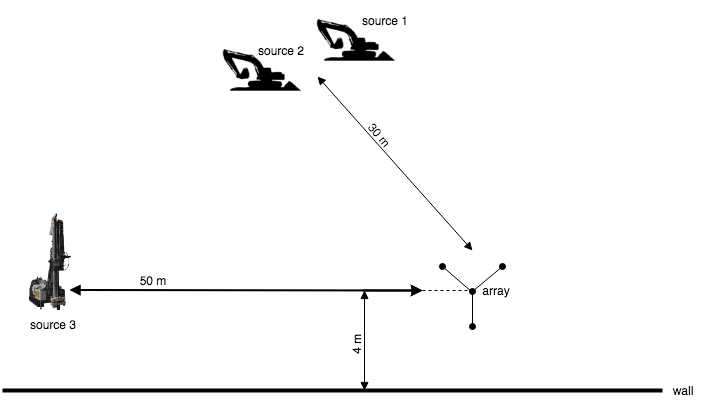
\includegraphics[width=0.8\textwidth]{Figures/scenario1diagram.png}
    \end{subfigure}
    \caption{Panorama of the construction field at the center point of the microphone array (top) and Top view schematic of the construction field (bottom)}
    \label{fig:Scenario2}
\end{figure}
\subsubsection{Results}
\begin{figure}[H]
    \centering
    \begin{subfigure}[b]{0.865\textwidth}
    \centering
    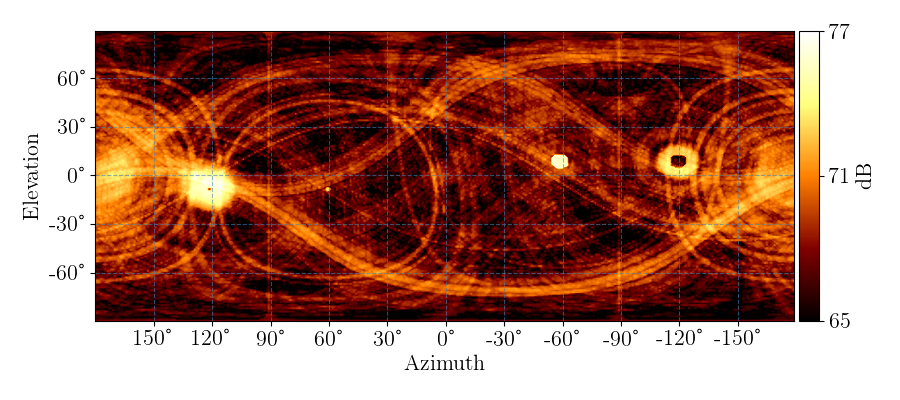
\includegraphics[width=0.865\textwidth]{Figures/construction1_normal.png}
\end{subfigure}
\vskip \baselineskip
\begin{subfigure}[b]{0.865\textwidth}
    \centering
    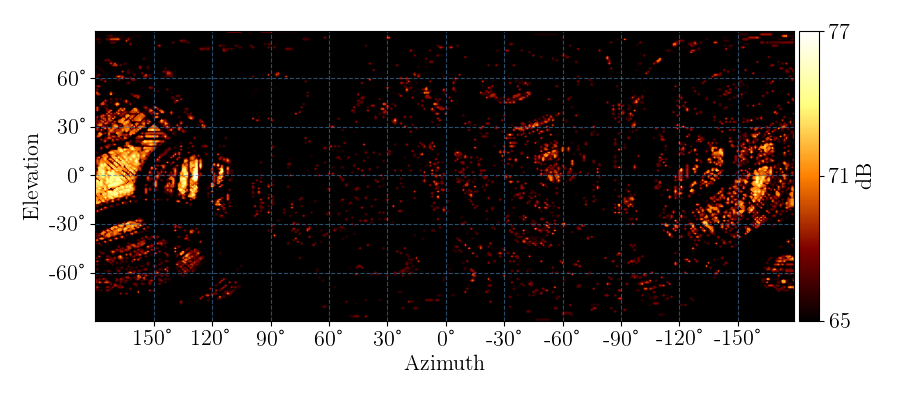
\includegraphics[width=0.865\textwidth]{Figures/construction1_minPow.png}
\end{subfigure}
\caption{Figures depict from top-to-bottom SRP-PHAT and minimum power SRP-PHAT localization for two construction machines located between (120$\degree$,0$\degree$) and (150$\degree$,0$\degree$) working in a construction field. A tapping machine is also making sound at (180$\degree$,<0$\degree$).}
\label{Fig:OutdoorLast1Src}
\end{figure}
\begin{figure}[H]
    \centering
    \begin{subfigure}[b]{1\textwidth}
    \centering
     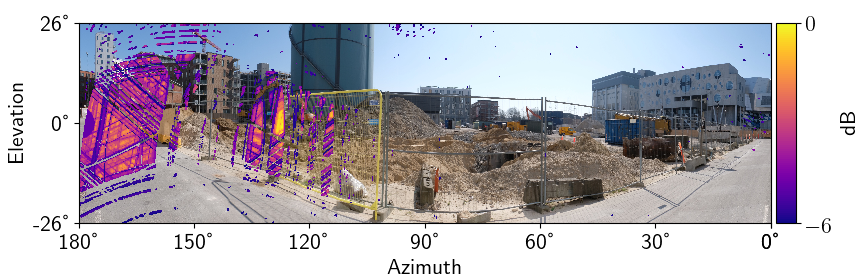
\includegraphics[width=1\textwidth]{Figures/Scenario1DYN6.png}
\end{subfigure}
\vskip \baselineskip
\begin{subfigure}[b]{1\textwidth}
    \centering
    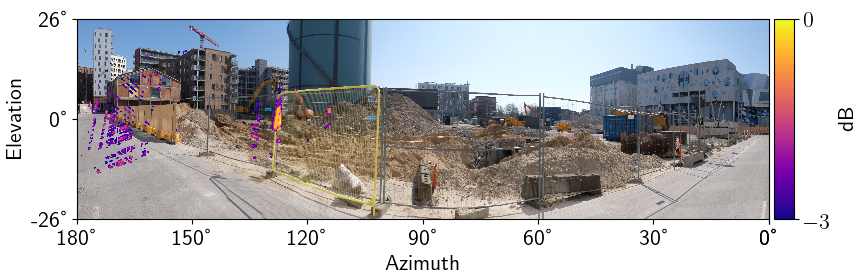
\includegraphics[width=1\textwidth]{Figures/Scenario1DYN3.png}
\end{subfigure}
\caption{Figures depict from top-to-bottom Min SRP-PHAT with dynamic range of 6dB and 3dB}
\label{Fig:Outdoorpicfull}
\end{figure}
\begin{figure}[H]
\vskip \baselineskip
\begin{subfigure}[b]{1\textwidth}
    \centering
    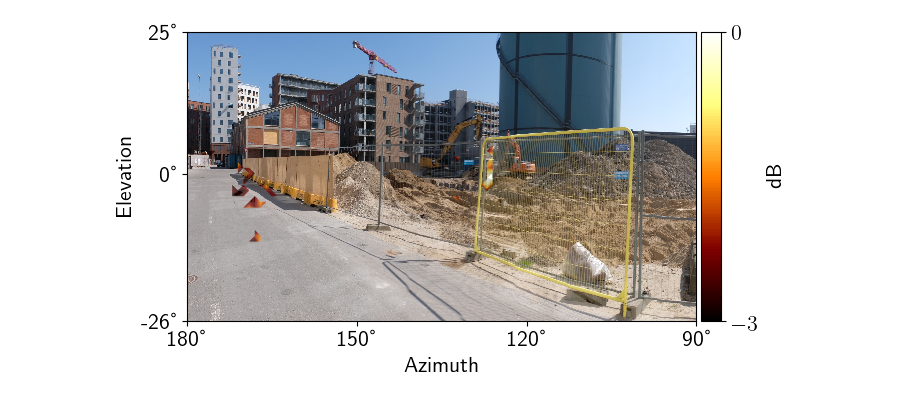
\includegraphics[width=0.9\textwidth]{Figures/Scenario1DYN3Zoomed.png}
\end{subfigure}
\caption{Zoomed figure depict from top-to-bottom Min SRP-PHAT with dynamic range of 3 dB}
\label{Fig:Outdoorpicfull}
\end{figure}
As can be seen the overlaid results are not precise. In fact, capturing and overlaying panoramic pictures correctly is not a trivial task. Depending on the number of pictures the camera takes when rotated about its sensor, angle skews can happen. Also depending on the speed at which the camera is rotated, these angle skews can be variable through the image. The correct way when capturing panoramic images is to use a fish-eye camera so that the entire panorama can be captured in a single image. However, since, such a setup was not available to the authors, the overlaid results from here on are not shown as panoramas, but as single shots taken with the camera pointed at the source.
\subsection{Sport event with crowd and PA system }
Measurements were performed during a sport competition outside, two main noise sources are present. The first one was a distributed PA system that covers all the zone as shown in figure \ref{fig:Scenario1diagram}, the second one was a crowd at (0°,0°), however the crowd level was quite low compared to the music level.
\begin{figure}[H]
    \centering
    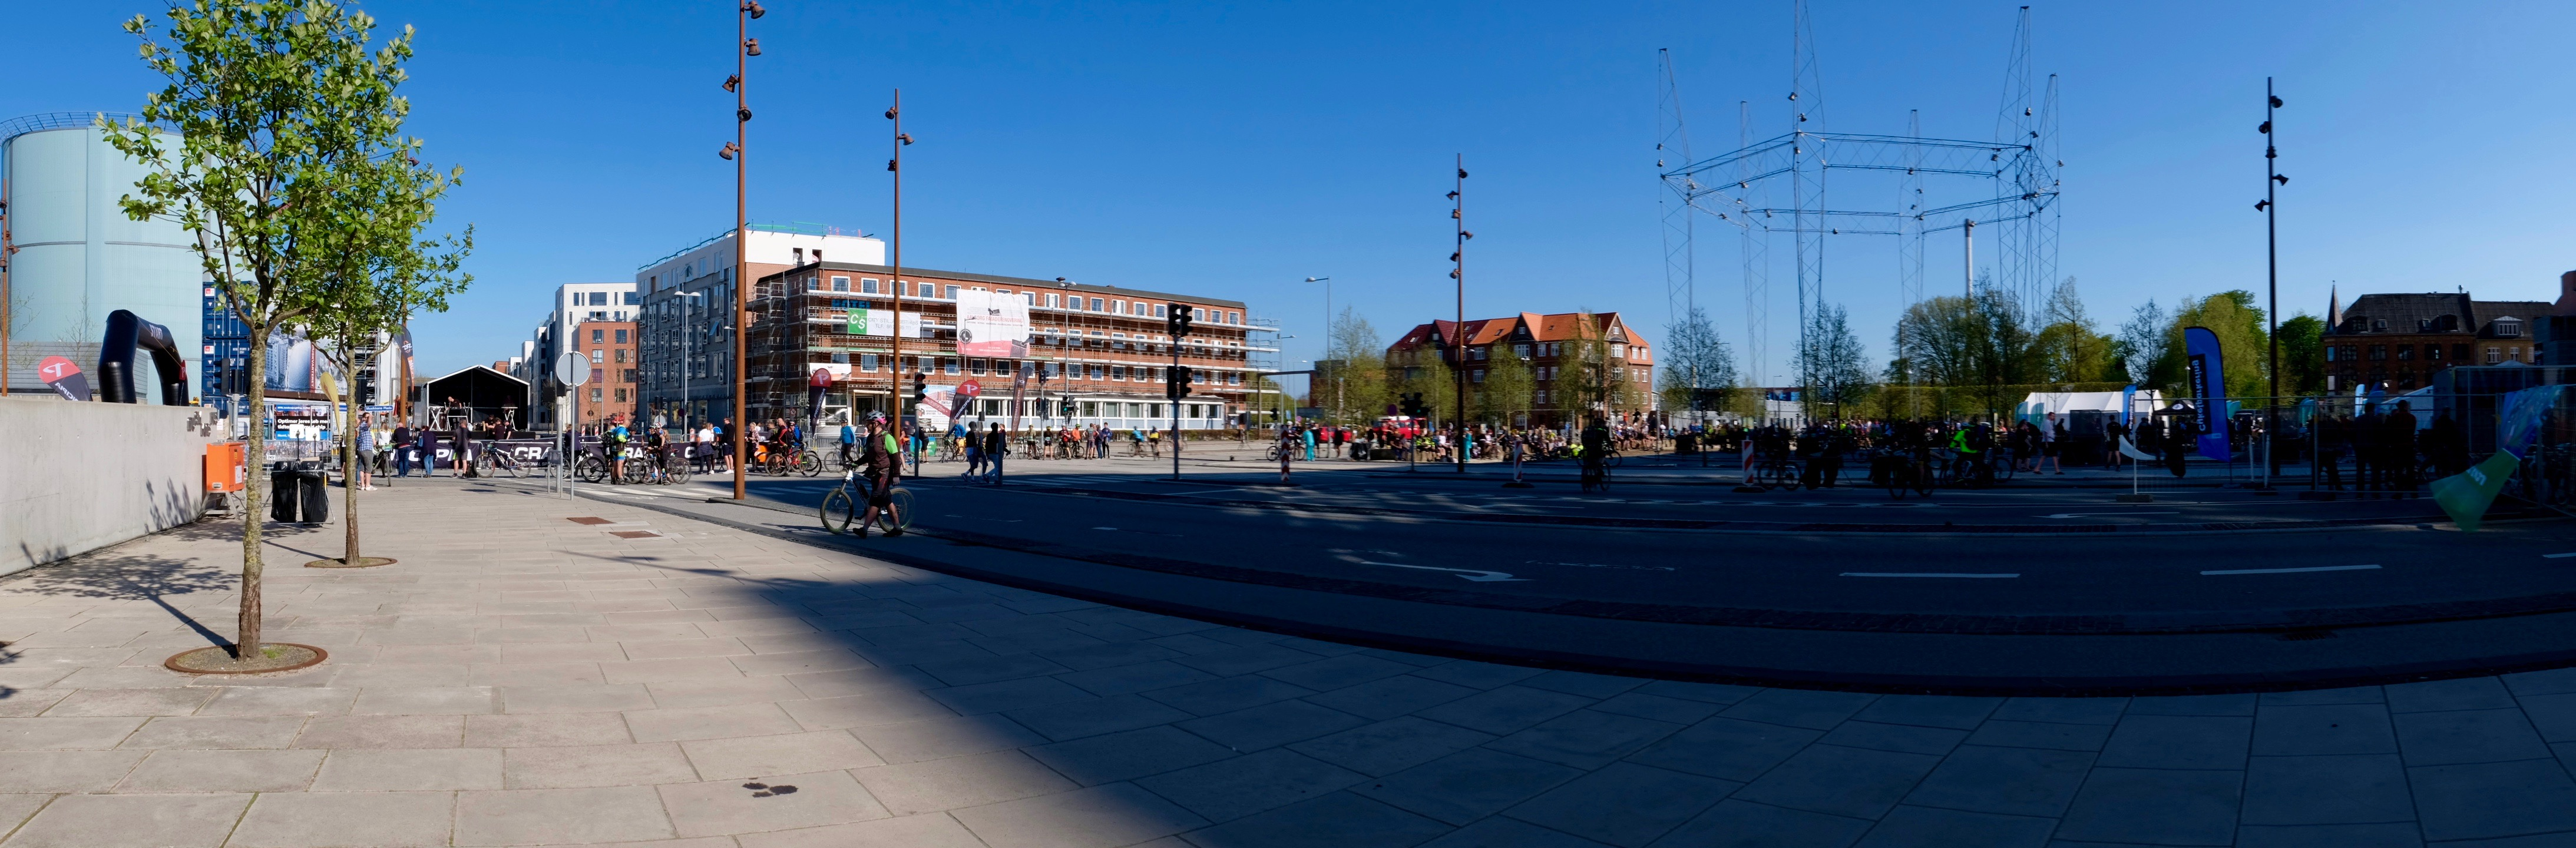
\includegraphics[width=1\textwidth]{Figures/bmxracepic.jpg}
    \caption{Panorama of the setup at the center point of the microphone array}
    \label{fig:Scenario3}
\end{figure}
\begin{figure}[H]
    \centering
    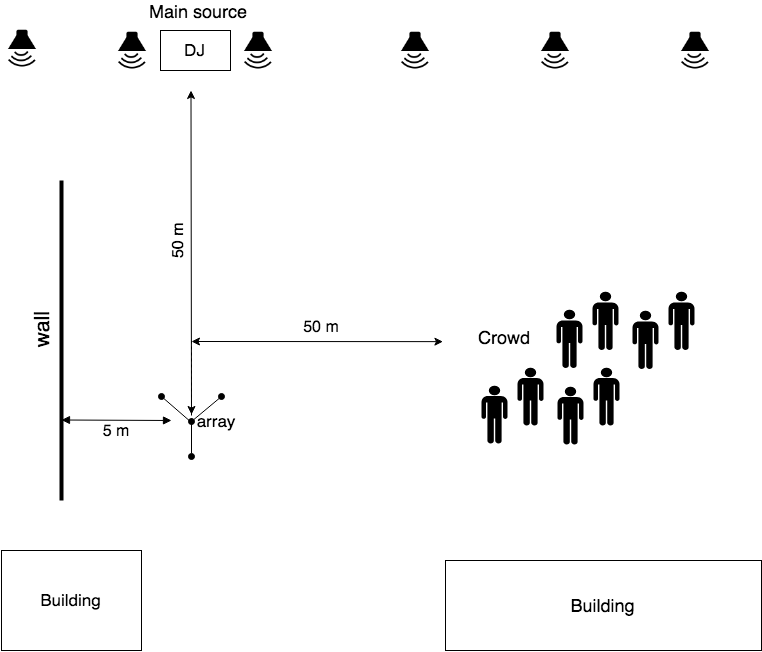
\includegraphics[width=0.8\textwidth]{Figures/bmxrace1.png}
    \caption{Top view of the scenario}
    \label{fig:Scenario1diagram}
\end{figure}
\subsubsection{Results}
\begin{figure}[H]
    \centering
    \begin{subfigure}[b]{1\textwidth}
    \centering
    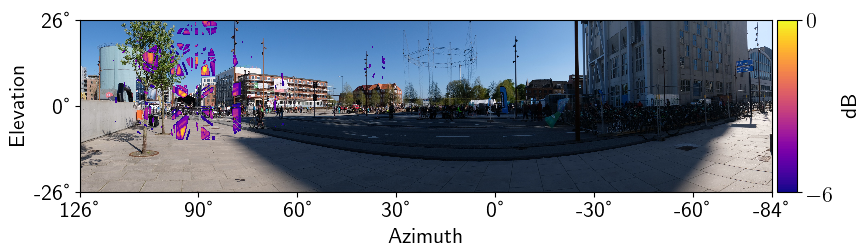
\includegraphics[width=1\textwidth]{Figures/BMX_1_6.png}
\end{subfigure}
\vskip \baselineskip
\begin{subfigure}[b]{1\textwidth}
    \centering
    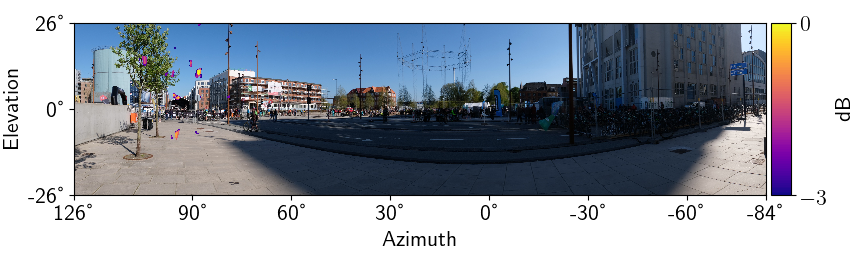
\includegraphics[width=1\textwidth]{Figures/BMX_1_3.png}
\end{subfigure}
\caption{Figures depict from top-to-bottom Min SRP-PHAT with dynamic range of 6dB and 3dB}
\label{Fig:bmxracedyn}
\end{figure}
\begin{figure}[H]
    \centering
    \begin{subfigure}[b]{1\textwidth}
    \centering
    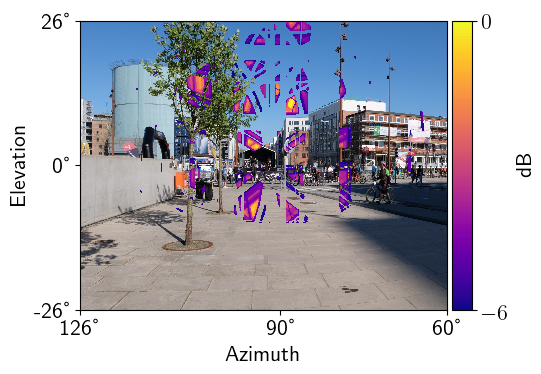
\includegraphics[width=1\textwidth]{Figures/BMX_1_6_zoomed.png}
\end{subfigure}
\vskip \baselineskip
\begin{subfigure}[b]{1\textwidth}
    \centering
    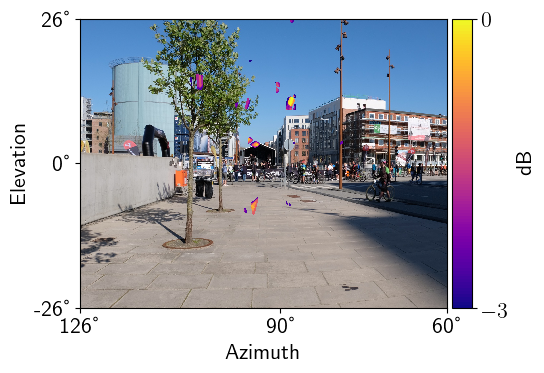
\includegraphics[width=1\textwidth]{Figures/BMX_1_3_zoomed.png}
\end{subfigure}
\caption{Figures depict from top-to-bottom Min SRP-PHAT with dynamic range of 6dB and 3dB}
\label{Fig:bmxracezomm}
\end{figure}
As can be seen the results are not good. Based on these results, the localization performance of the algorithm was simulated when multiple sources were playing the same sound (Sec. \ref{sec:Coherent}). It was found that when multiple coherent sources are present, the algorithm can fail as the constant phase difference between the multiple sources can be detected as a pseudo-source. 
\subsection{Outdoor concert}
Measurements were performed during an outdoor concert where a DJ was playing music on a PA system. The PA system was composed of two tops and one sub. The setup can be seen in figure \ref{fig:Scenario4}
\begin{figure}[H]
    \centering
    \includegraphics[width=1\textwidth]{Figures/P4day.jpg}
    \caption{Picture of the setup at the center point of the microphone array}
    \label{fig:Scenario4}
\end{figure}
\subsubsection{Results}
\begin{figure}[H]
    \centering
    \begin{subfigure}[b]{1\textwidth}
    \centering
    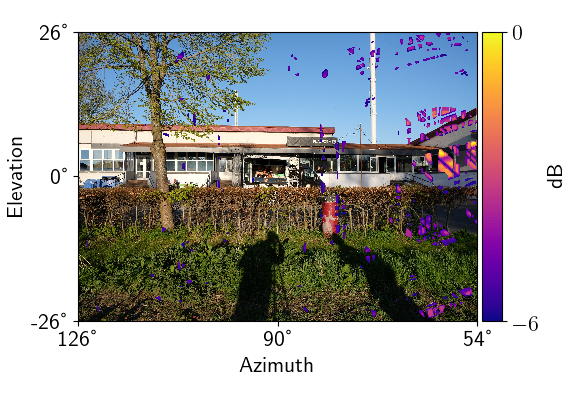
\includegraphics[width=1\textwidth]{Figures/P4_Day_6.png}
\end{subfigure}
\vskip \baselineskip
\begin{subfigure}[b]{1\textwidth}
    \centering
    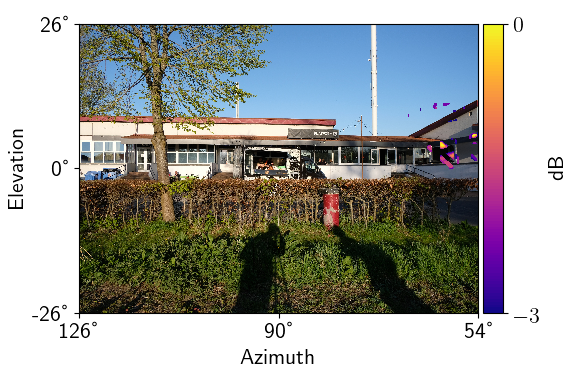
\includegraphics[width=1\textwidth]{Figures/P4_Day_3.png}
\end{subfigure}
\caption{Figures depict from top-to-bottom Min SRP-PHAT with dynamic range of 6dB and 3dB(Zoomed)}
\label{Fig:P4Day}
\end{figure}
\subsection{Indoor concert}
Measurements were made of a concert happening indoors. The event took place at midnight, however the photo was taken during the day so that the overlay is easier to see.
\begin{figure}[H]
    \centering
    \begin{subfigure}[b]{1\textwidth}[H]
    \centering
    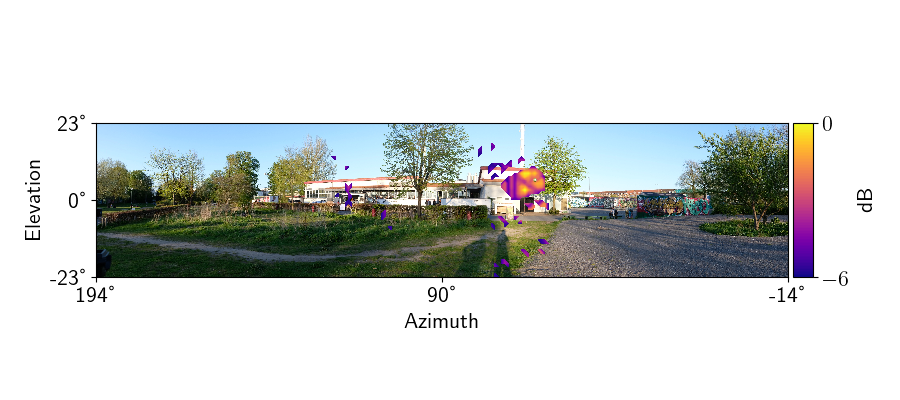
\includegraphics[width=1\textwidth]{Figures/P4Night6dB.png}
\end{subfigure}
\vskip \baselineskip
\begin{subfigure}[b]{1\textwidth}[H]
    \centering
    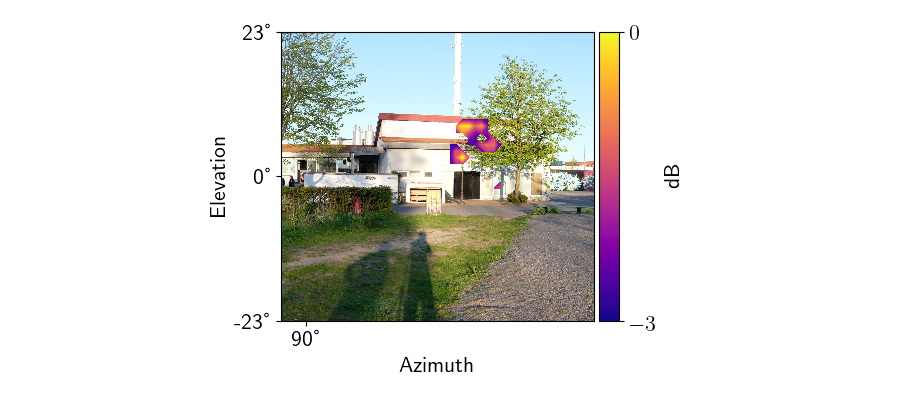
\includegraphics[width=1\textwidth]{Figures/P4Night3dB_Zoomed.png}
\end{subfigure}
\caption{Figures depict from top-to-bottom Min SRP-PHAT with dynamic range of 6dB and 3dB(Zoomed)}
\label{Fig:P4Night}
\end{figure}
\subsection{Roadside noise}
Cars passing through a crossing were measured in a close range ($2-10m$). A single loud motorcycle passing through was measured.
\subsubsection{General traffic}
\subsubsection{Loud motorcycle}
\subsection{Chalk mine}
A chalk mining machine was measured from a large distance ($500m$), with different microphone aperture sizes. The same measurement was then run closer ($100m$) and even closer ($90m$).
\subsection{Lookout large aperture}
\begin{figure}[H]
    \centering
    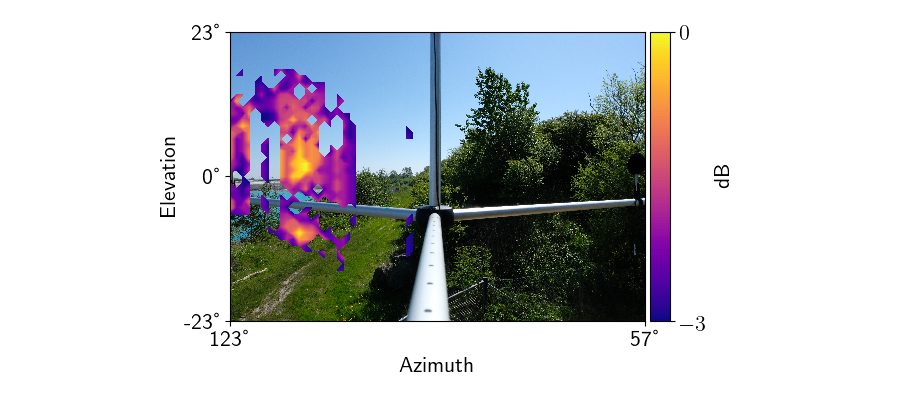
\includegraphics[width=1\textwidth]{Figures/ChalkFarFar.png}
    \caption{Localization results of the chalk mine from a far away lookout close to traffic noise}
    \label{fig:ChalkCLose}
\end{figure}
%\subsubsection{Lookout small aperture}
\subsubsection{Close to mine, far from edge}
\begin{figure}[H]
    \centering
    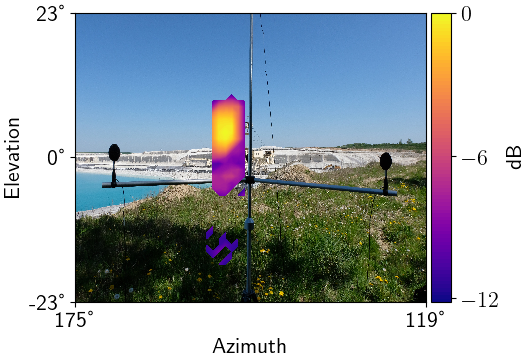
\includegraphics[width=1\textwidth]{Figures/ChalkFar.png}
    \caption{Localization results of the chalk mine far from the edge}
    \label{fig:ChalkCLose}
\end{figure}
\subsubsection{Close to mine, close to edge}
\begin{figure}[H]
    \centering
    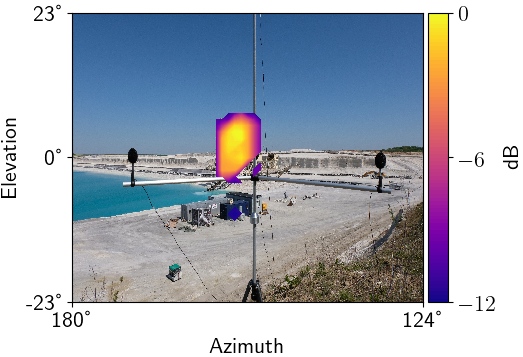
\includegraphics[width=1\textwidth]{Figures/ChalkClose.png}
    \caption{Localization results of the chalk mine close to the edge}
    \label{fig:ChalkCLose}
\end{figure}

